\chapter{Technology and Software}

\section{Android OS}
Android is a Linux based operating system primarily designed for touchscreen devices such as smartphones and tablets. It is developed by Google and is supported by The Open Handset Alliance (OGHA). The source code was released as open source under the Apache License, and The Android Open Source Project is tasked with maintaining and further developing the operating system. The OGHA is a consortium focused on developing open standards for mobile devices, and members of the consortium are not allowed to produce phones that are not compatible with the Android OS. Applications for the Android OS are primarily written in a customized version of Java using the Software Development Kit, but it is possible to partly write applications in C and C++ using the Native Development Kit. 

Given that the Android OS code is open source and highly modifiable both the community and smartphone distributors have taken advantage of this. Distributors such as HTC and Samsung have both made their modifications to the Android OS. The modifications are primarily focused on making the user interface more powerful and user friendly in order to enhance the user experience\cite{htcSense}. The Android Community has taken this further by developing their own versions of the Android "firmware" or "ROM" that is intended as a replacement for the stock firmware. This firmware might be specialized to be light weight, or allow a high degree of customization. to better suit the user. The most well known community firmware being the CyanogenMod \cite{cyanogenMod}. In order to install and use custom firmware a user needs to "root" the phone, by rooting the phone the user gains access to the entire system, giving him the ability to delete and alter system critical files.

The software center for Android is known as "Google Play" and allows developers to easily distributed their applications. Users can then choose and download thousands of applications, some are free, while others have to be paied for. The idea is that as long as a device runs the Android OS it can run any of the applications on Google Play. The first Android device was sold in October 2008. By the end of 2010 the Android OS had become the leading smartphone platform \cite{androidLeadingPlatform}, and at the second quarter of 2012 it had a worldwide smartphone market share of 68\%\cite{androidMarketShare}. During the third quarter of 2012 500 million devices had been activated and there are approximately 1.3 million activations per day \cite{androidDevices}. Currently the newest version of Android is version 4.1 codename Jelly Bean. The first version to be released was version 1.5 in 2009 \cite{cupcake} codenamed Cupcake. With each new version of Android the developer API is improved and functionality is added. Applications using a lower API level developed for earlier Android versions can run on higher API levels, but not the other way around. Using a lower level API allows an application to support more devices, but sacrifices added features and optimization located in a higher level API.

\begin{figure}[h!]
  \centering
    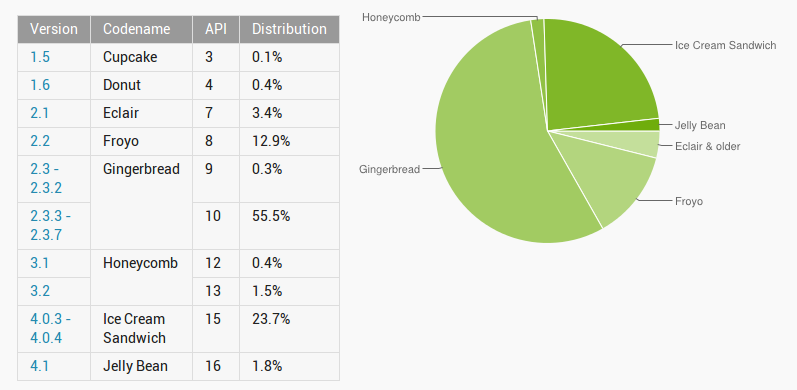
\includegraphics[width=1.0\textwidth]{androidVersionDistribution.png}
    \caption{\footnotesize The data is based on Android devices that accessed Google Play during a 14 day periode ending on October 1, 2012 \cite{androidVersions}}
\end{figure}


\subsection{Architecture}
Older Android versions are based on Linux kernel 2.6 while Android version 4.0 and higher use Linux kernel 3.0. Google has made alternations to the standard Linux kernel by not including all the standard libraries, this makes porting existing Linux desktop applications difficult. The kernel interacts with the hardware and contains all the necessary drivers in order to do so. As the operating system was designed to run on a variety of hardware, and the kernel functions as an abstraction layer between the hardware and software in addition to handling the standard kernel tasks such as resource management, networking and security.

The library layer contains the native android libraries that enable android devices to handle different types of data. The libraries are written in c++ or c and are hardware specific. These libraries can be accessed through the use of the Android NDK and is recommended for functionality not attainable through the standard SDK. There are dozen of native libraries but some of them include: Webkit is the browser engine used to display HTML content, SQLite is used for data storage locally on the device, OpenGL to render 2D and 3D graphics, in addition to several media codecs.Google has developed their own Java Virtual Machine called the Dalvik Virtual Machine. It runs Android applications and is optimized for low memory and low processing power environments. It provides most of the same features as the JVM such as isolation, multi-threading and memory management. The DVK in addition to core java libraries are considered to be the Android Runtime.

The Application framework level is what applications on the Android device interact with. Developers use the programs located in this framework as tools to build their own applications on. These programs provide access to and manage basic phone functions, such as gps tracking (Location manager), sharing data between applications(Content Providers) voice calls (Telephone Manager), applications lifecycles (Activity Manager) and so on. Any application installed by the user is located in the top application layer. These are applications created by developers and can range from sms clients, to 3D games. As long as the user permits it and the hardware can handle it the applications can be programmed to do anything.


\begin{figure}[!h]
  \centering
    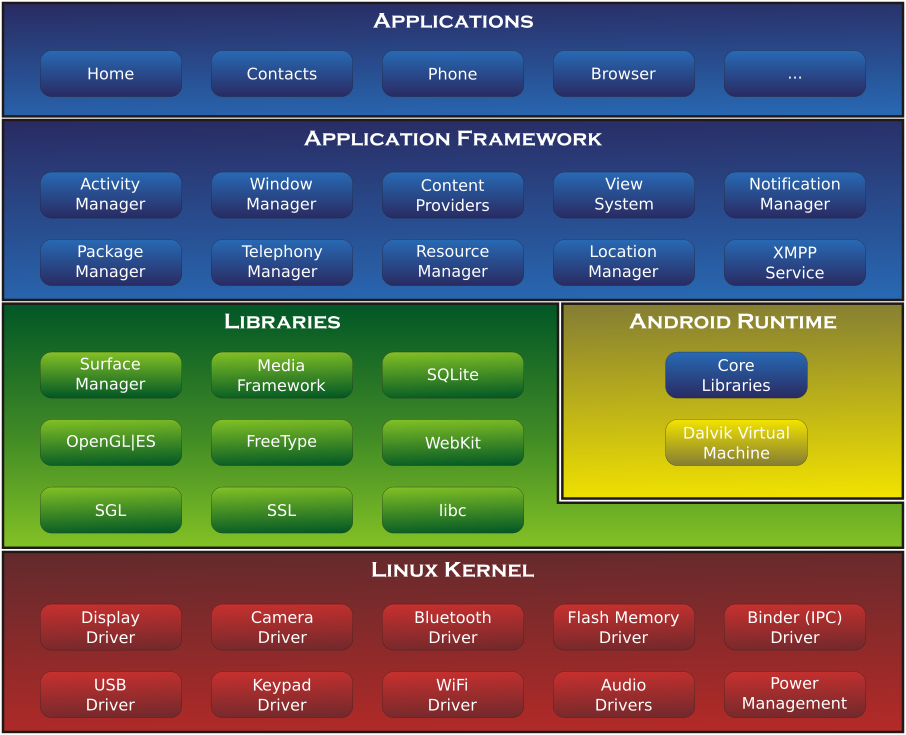
\includegraphics[width=.70\textwidth]{androidArchitecture.png}
    \caption{\footnotesize A visual representation of the Android architecture}
\end{figure}


\section{Java}
Is it neccessary to write something aobut Java?

\section{PS3 Move}

\subsection{Motion Controller Hardware}
The PS Move motion controller contains advanced motion sensing, making it an ideal peripheral for a bio-feedback system. It features motion tracking through a three axis accelerometer, a three axis angular rate sensor and provides location tracking through the built in magnetometer. The built in vibration could be used to provide feedback to the user \cite{psMoveTech}.

\subsection{PS Move API}

The PS Move API \cite{PSMoveAPI} is written in C, but contains bindings for various languages, including Java and C\# which are both languages used in smartphone application development. The API explicitly mentions that it runs on Android devices. This is a truth with modifications. It will not run out of the box on an Android device, in addition restructuring and heavy modification of the Android device is required.  The Android OS runs on top of a modified Linux kernel, this kernel does not contain the necessary libraries and drivers in order for the API and Motion controller connectivity to function properly. %Does this need citation?
The next step would be to compile the C API into a shared library using the Android NDK, and use the shared library Java bindings in the Android Java code.

Everything is possible with enough time, but given the time constraint and amount of time required to get this running it was decided that this was not a path worth pursuing for this project. With some much work required it would be simpler to run Ubuntu off an Android device if this becomes available in the future. \cite{ubuntuAndroid}

\section{Wii Remote with Motion Plus}

\subsection{Wii Remote and Motion Plus Hardware}
The original Wii Remote features motion tracking for vertical movement, left-right horizontal movement, and horizontal rotation through the use of an ADXL330 accelerometer.\cite{wiiAccelerometer}.
In June 2009 Nintendo released the Wii MotionPlus expansion device which contains a dual-axis tuning fork and a single-axis gyroscope\cite{wiiMotionPlus}.
The expansion device improves the motion tracking of the Wii Remote greatly, but makes it larger. Nintendo has now started selling the Wii Remote Plus. It is the same size as the Wii Remote, but has the Wii MotionPlus already built in. Both of the controller types have the ability to provide vibration and basic audio feedback.

%%WRITE SOMETHING ABOUT THE NUNCHUCK?

\subsection{Wii Remote API}
At time of writing no Wii Remote library has been created for the Android OS. Though there are plenty of Wii remote libraries out there none of them are intended to be used on android devices. This section will cover the most developed liberalities that are implemented in Java.

\subsubsection{WiiRemoteJ}
WiiRemoteJ is one of the most complete libraries for the Wii remote. It is a pure Java library with support for a large amount of Wii extensions such as the Wii Guitar, and Wii Balance Board. It does however lack support for the MotionPlus extension. The library has not been update since July 2008. The author has taken down the homepage where the library was originally located, but it can be found on third party websites. \cite{WiiRemoteJ}

\subsubsection{WiiuseJ}
WiiUseJ is a lightweight Java API. It was built on top of the Wiiuse API and only supports the Wii Remote and the Nunchuck. Like the previous library it lacks support for the MotionPlus extension. The project has been discontinued since January 2009. \cite{Wiiusej}

\subsubsection{Motej}
Motej is an open source (licensed under ASL 2.0) library for the Wii remote written in Java. Motej supports only the Wii Remote and IR Camera in it's basic form, but the extras library adds support for the balance board, classic controller, and nunchuk. The project is currently at version 0.9, but was discontinued in 2009. \cite{Motej}

\subsection{Bluetooth}
%General information about bluetooth, and some text about L2CAP and why Android sucks.
Bluetooth is a widely used wireless communication technology for shorter distances. Due to its low power consumption and low cost is has become one of the leading standards in its field and is supported by most modern operating systems, either through integrated hardware or through portable Bluetooth adapter. Most, if not all, modern phones come with a built-in Bluetooth card/radio. %CITATION BITCHES! 
The Wii Remote uses Bluetooth to communicate wirelessly with other devices, using the logical link control and adaptation protocol (L2CAP). 
